\documentclass[]{article}
\usepackage[T1]{fontenc}
\usepackage{lmodern}
\usepackage{amssymb,amsmath}
\usepackage{ifxetex,ifluatex}
\usepackage{fixltx2e} % provides \textsubscript
% use upquote if available, for straight quotes in verbatim environments
\IfFileExists{upquote.sty}{\usepackage{upquote}}{}
\ifnum 0\ifxetex 1\fi\ifluatex 1\fi=0 % if pdftex
  \usepackage[utf8]{inputenc}
\else % if luatex or xelatex
  \ifxetex
    \usepackage{mathspec}
    \usepackage{xltxtra,xunicode}
  \else
    \usepackage{fontspec}
  \fi
  \defaultfontfeatures{Mapping=tex-text,Scale=MatchLowercase}
  \newcommand{\euro}{€}
\fi
% use microtype if available
\IfFileExists{microtype.sty}{\usepackage{microtype}}{}
\usepackage[margin=1in]{geometry}
\usepackage{graphicx}
% Redefine \includegraphics so that, unless explicit options are
% given, the image width will not exceed the width of the page.
% Images get their normal width if they fit onto the page, but
% are scaled down if they would overflow the margins.
\makeatletter
\def\ScaleIfNeeded{%
  \ifdim\Gin@nat@width>\linewidth
    \linewidth
  \else
    \Gin@nat@width
  \fi
}
\makeatother
\let\Oldincludegraphics\includegraphics
{%
 \catcode`\@=11\relax%
 \gdef\includegraphics{\@ifnextchar[{\Oldincludegraphics}{\Oldincludegraphics[width=\ScaleIfNeeded]}}%
}%
\ifxetex
  \usepackage[setpagesize=false, % page size defined by xetex
              unicode=false, % unicode breaks when used with xetex
              xetex]{hyperref}
\else
  \usepackage[unicode=true]{hyperref}
\fi
\hypersetup{breaklinks=true,
            bookmarks=true,
            pdfauthor={Andresa de Andrade},
            pdftitle={Assignment 1},
            colorlinks=true,
            citecolor=blue,
            urlcolor=blue,
            linkcolor=magenta,
            pdfborder={0 0 0}}
\urlstyle{same}  % don't use monospace font for urls
\setlength{\parindent}{0pt}
\setlength{\parskip}{6pt plus 2pt minus 1pt}
\setlength{\emergencystretch}{3em}  % prevent overfull lines
\setcounter{secnumdepth}{5}

\title{Assignment 1}
\author{Andresa de Andrade}
\date{October 4, 2015}

\begin{document}

\begin{center}
\huge Assignment 1 \\[0.2cm]
\end{center}
\begin{center}
\large \emph{Andresa de Andrade}\\[0.1cm]
\end{center}
\begin{center}
\large \emph{October 4, 2015} \\
\end{center}
\normalsize


{
\hypersetup{linkcolor=black}
\setcounter{tocdepth}{2}
\tableofcontents
}
\section{Abstract}\label{abstract}

In recent years, it's become important to understand the factors that
lead a buyer to finalize a conversion within the online marketing
business. Therefore the purpose of this project is to understand any
possible pattern in the customer behavior of an online shop and try to
predict the types of coupons that the customers would want to use/buy.

Along our way we shall demonstrate the structure of categorization and
how a machine learning algorithm would work for this particular case. We
will also present the conditions assumed in order to have the model
working properly. And the facts ignored but also important to a
thoroughly analysis.

We will also show the evaluation methods between the different
methodologies here presented.

\section{Introduction}\label{introduction}

In this paper and the follow documents presented along the way of this
project, we will attempt to demonstrate if the online browsing history
is correlated to final purchase.

In that case, we will be using four data files to learn from. The first
file is composed with the list of 22.874 customers and some personal
information that will be described in the dataset section. The second
file to be used is a file that contains information related to users
buying voucher. And the third file to be used contain the data related
to users browsing in the site. The last file to be used is the coupon
detail information that contains all the data specifically about the
coupon.

\section{Related Research}\label{related-research}

There are several researches and projects done related to online
customer behavior and coupon usage.

\begin{itemize}
\item
  Blattberg et al. (1978) suggested that the coupon usage would be
  related to demographics characteristics where the consumers are
  assumed to minimize the sum of transaction costs, storage costs and
  the price of the item. He basically suggested that the upper income
  households, the more likely to redeem the coupon.
\item
  Narasimhan (1984) proposed that intensity of coupon usage is related
  inversely to a household's opportunity cost of time. Therefore it
  would be expected that in households that are more educated, have
  children under six and husband and wife are employed would have a
  lower prone to use coupons.
\item
  Bawa and W. Shoemaker (1987) suggested that the intention of using the
  coupon (which in their project is called CPI - coupon proneness index)
  is a function of household characteristics and customer behavior.
\end{itemize}

-Kwon Jung (2010) suggested that the online usage of coupon is a funcion
of the percentage of discount offered and demographics.

\section{Dataset}\label{dataset}

As mentioned before, the dataset used is composed by 4 files and they
all have an entity in common. Above you can see the ER diagram for the
data.

\begin{figure}[htbp]
\centering
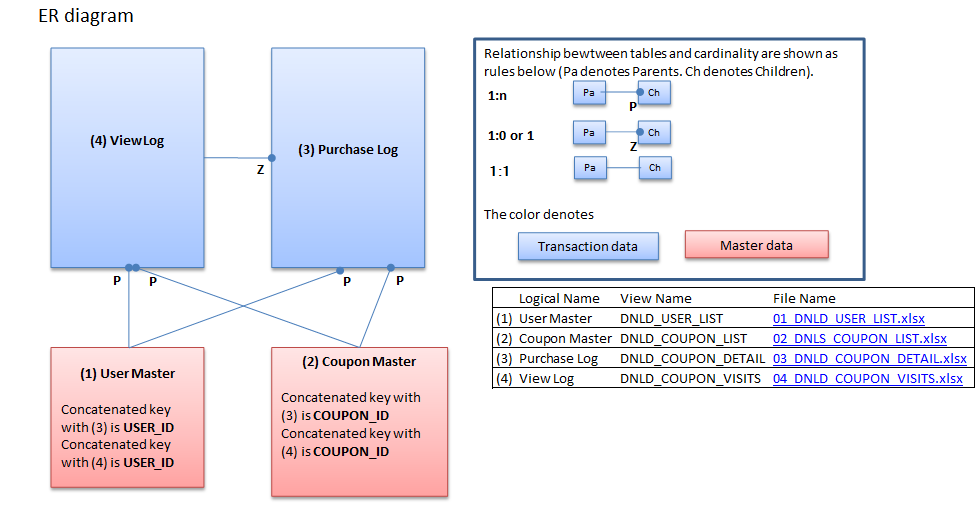
\includegraphics{erdiagram.png}
\caption{ER Diagram}
\end{figure}

\begin{itemize}
\itemsep1pt\parskip0pt\parsep0pt
\item
  user\_list.csv: contains 6 features and 22,873 users. The features are
  related to (registered day, gender, age, date that unregistered,
  preferable name and user id).
\item
  coupon\_detail.csv: contains 6 features and 168,997 entries. The
  columns consist in information about quantity bought, purchase date,
  geographic area that was bought, purchase identifier, user id and
  coupon id.
\item
  coupon\_visits.csv: contains 8 features that refer manly to the
  browsing logs. The columns are purchase flag, purchase id in case it
  happened, log date, page serial, refer, coupon id, user id, session
  id.
\item
  coupon\_list.csv contains 24 features related to the coupon like
  category, expire date, what week days it's available, discount value,
  and so on.
\end{itemize}

\section{Analysis}\label{analysis}

In our process to model the data we will have 4 main steps.

\begin{itemize}
\itemsep1pt\parskip0pt\parsep0pt
\item
  Data preparation: where will merge/join the tables creating one single
  table to be used. In addition we will check if there is any missing
  information or data that should be transformed.
\item
  Descriptive Analysis: where we will calculate basic statistics to
  understand how the data is distributed.
\item
  Modeling: where the methodology will be tested in order to predict the
  coupon usage.
\item
  Data Evaluation: the models will be compared and testes against each
  other in order to choose the best one.
\end{itemize}

\subsection{Data Preparation}\label{data-preparation}

In order to run our model we will tread the dataset to have one flat
table containing only users that had at least one interaction in the
website and with the following features:

\begin{enumerate}
\def\labelenumi{\arabic{enumi})}
\item
  purchaseflag: 1 or 0 variable containing 1 if purchase was made and 0
  otherwise
\item
  age
\item
  price\_rate: where it holds the percentage of discount that the
  customer can have
\item
  unique\_referrer: how many referrers that user had before purchased
  something.
\item
  sessions: number of sessions prior to a purchase.
\item
  usable\_date: days of the week that the coupon visited was available
  to be used.
\item
  city that the coupon was available to be used
\item
  business the coupon was available to be used.
\end{enumerate}

As result we had a flat table with 2 million of interactions and
therefore I selected 30 thousand interactions for this work.

Due the reasonable amount of data, we will separated the flattened table
in 80\% for the training and 20\% for the testing and model evaluation.

And the train data will be used with a cross validation approach.

\subsection{Methodology}\label{methodology}

Looking back at the goal of this project, it consisted in predict online
coupon usage based on customer behavior.

1 - The data was transformed into portions that can be workable using
our model (Logistic Regression)

2 - The data was spitted in 2, the train (80\% or 24k interactions) and
the test (20\% or 6k interactions)

3 - The train data was spitted in 10 folds and the model was designed to
each one of the folder and tested in the complimentary data.

4 - To select the best fitted model we used AUC or RoC as a criteria

5 - The model was then applied to the test dataset.

You can find the code to transform the data in this link:

``library(''RWeka``) \# for datasets library(''ROCR``) \# visualize
performance of classifiers library(''caret``) \# for confusion matrix
library(''e1071``) \# may be needed for caret

sample\_1\textless{}-read.csv(`no\_referrers.csv')

sample\_1$price_rate<-as.numeric(sample_1$price\_rate)
sample\_1$age<-as.numeric(sample_1$age)
sample\_1$item_count<-as.numeric(sample_1$item\_count)
sample\_1{[},6{]}\textless{}-as.numeric(sample\_1{[},6{]})

features =
paste(names(sample\_1{[}2:length(names(sample\_1))-1{]}),collapse =
``+'') formula\_text \textless{}-
paste(names(sample\_1{[}1{]}),``\textasciitilde{}'', features) formula
\textless{}- as.formula(formula\_text)

rn\_train \textless{}- sample(nrow(sample\_1),
floor(nrow(sample\_1)*0.8)) folds \textless{}-
createFolds(sample\_1\$purchase\_flag)

i = 1 for (f in folds)\{ train \textless{}- sample\_1{[}-f,{]}
cross\_validation \textless{}- sample\_1{[}f,{]}

fit \textless{}- glm(formula,data=train,family=binomial()) print(i)
print(summary(fit))
cross\_validation$scores <- predict(fit, type="response",                        newdata=cross_validation)   pred<-prediction(cross_validation$scores,
cross\_validation$purchase_flag)   c <- confusionMatrix(as.integer(cross_validation$scores
\textgreater{} 0.2), cross\_validation$purchase_flag)   c$table

\#writes chart perf\textless{}-performance(pred,``tpr'',``fpr'')
\#plot\_name = paste(``output/RoC'', i, ``.png'')
\#png(filename=plot\_name) \#plot\_title = paste(``cross\_validation'',
i) \#plot(perf, lty=1, main = plot\_title)

\# test\$scores \textless{}- predict(fit, type=``response'', \#
newdata=test)

\# pred\textless{}-prediction(test$scores, test$purchase\_flag) \#
perf\_test\textless{}-performance(pred,``tpr'',``fpr'') \# plot\_name =
paste(``output/test\_RoC'', f, ``.png'') \# png(filename=plot\_name)\\
\# plot(perf\_test, lty=1, main = ``Test Validation'') i = i + 1

\}"

\subsection{Model Evaluation}\label{model-evaluation}

The model evaluation consists in RoC and AuC as a good evaluation for
logistic regression.

\section{References}\label{references}

\begin{itemize}
\item
  Online vs.~Offline Coupon Redemption Behaviors Kwon Jung 2010
\item
  The Coupon Prone Consumer: Some Findings Based on Purchase Behavior
  across Product Classes.
\item
  Evaluating Logistic Regression at
  \url{http://www.r-bloggers.com/evaluating-logistic-regression-models/}
\item
  Tools for Machine learning at
  \url{http://aimotion.blogspot.ca/2010/08/tools-for-machine-learning-performance.html}
\end{itemize}

\end{document}
